% vim: tw=80

\chapter{PDF Constraints of the Triple-Differential Dijet Measurement}
\label{sec:pdf_constraints}

In many precision measurements at the LHC, the proton PDFs are an essential
ingredient. As the PDFs cannot be calculated from perturbative QCD, they are
derived from experimental data of collider and fixed-target experiments.
Deep-inelastic scattering (DIS) data from the HERA collider cover most of the
kinematic phasespace. The triple-differential dijet cross section contains
additional information in the high-$x$ region and can constrain the PDFs, in
particular the gluon PDF. 

\section{The HERAFitter Framework}
\label{section:herafittersetup}

The constraints of the triple-differential dijet measurement on the proton PDFs
is demonstrated by including the cross section measurement in a PDF fit in
combination with inclusive DIS cross sections from the HERA experiments. The
HERA-II DIS data were the basis for the determination of the HERAPDF 2.0 PDF
set.

HERAFitter is an open source framework to fit the PDFs to experimental data
based on the Dokshitzer-Gribov-Lipatov-Altarelli-Parisi
(DGLAP)~\cite{Gribov:1972ri,Altarelli:1977zs,Dokshitzer:1977sg} equations. To
ensure consistency between DIS and QCD calculations, the fits are performed at
NLO. The DIS cross sections are calculated by the QCDNUM
software~\cite{Botje:2010ay}.

The parametrization used in the PDF fit is based of the HERAPDF 2.0
parametrization and introduces additional terms which were found to better
describe the additional added jet measurement. The PDFs parameterization is
definded at the starting scale $Q_0$ set to $Q_0 = \SI{1.9}{\GeV \square}$ and
the five independent PDFs $xu_v(x)$, $xd_v(x)$, $xg(x)$, $x\bar{U}(x)$ and
$x\bar{D}(x)$ are parameterized as follows:

\begin{align}
  xg(x) &= A_g x^{B_g} (1-x)^{C_g} (1 + E_g x^2) - A'_g x^{B'_g} (1-x)^{C'_g} \\
  xu_v(x) &= A_{u_{v}} x^{B_{u_{v}}} (1-x)^{C_{u_{v}}}(1 + D_{u_{v}}x + E_{u_{v}}x^2)\\
  xd_v(x) &= A_{d_v} x^{B_{d_v}} (1-x)^{C_{d_{v}}}\\
  x\bar U(x) &= A_{\bar U} x^{B_{\bar U}} (1-x)^{C_{\bar U}}(1 + D_{\bar U}x)\\
  x\bar D(x) &= A_{\bar D} x^{B_{\bar D}} (1-x)^{C_{\bar D}}
\end{align}

Not all parameters are actually fitted. The normalization parameters $A_g$,
$A_{u_{v}}$ and $A_{d_{v}}$ are calculated using the QCD sum rules. $B_{\bar
U}=B_{\bar D}$ and $A_{\bar U} = A_{\bar D}(1-f_s)$ ensure the same
normalization for the $\bar u$ and $\bar d$ PDF for the $x \rightarrow 0$
region. The strangeness fraction is set to $f_s = 0.40$. The generalized-mass
variable flavour number secheme as described in
in~\cite{Thorne:1997ga,Thorne:2006qt} is used with the strong coupling constant
set to $\asmz= 0.1180$.


\subsection{Treatment of PDF uncertainties in the Fits}
\label{section:treatment_pdf_uncertainties}

The uncertainty of the PDFs is subdivided into three independent sources, which
are evaluated separately and finally added in quadrature to give the total
uncertainty.

\paragraph{Experimental Uncertainties} 
They result from propagated statistical and systematic uncertainties of the data
points and are propagated to the PDF using the Hessian eigenvector
method~\cite{Pumplin:2001ct}. The Hessian matrix is defined by the second
derivatives of the fitted PDF parameters at the \chisq minimum. The matrix is
diagonalized and the eigenvectors are computed, see
Fig.~\ref{fig:eigenvector_basis_set}. 

\begin{figure}[htb]
  \centering
  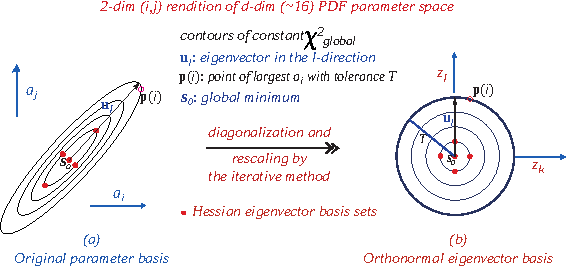
\includegraphics[width=1.0\textwidth]{figures/pdf_constraints/hessianmethod.pdf}
  \caption[Transformation of the parameter basis to the eigenvector basis.]
    {Transformation from the original parameter basis to the orthonormal
    eigenvector basis. The uncertainty on the PDF can be propagated to a
    physical quantity $X$ using these eigenvector PDF sets~\cite{Pumplin:2001ct}.}
    \label{fig:eigenvector_basis_set}
\end{figure}

Using an iterative method, the down- and upwards variation of each eigenvector
corresponding to $\chisq = \chisq_{\mathrm{min}} + 1$ is calculated. Since the
eigenvectors are orthogonal, the eigenvector variation PDFs correspond to
independent sources of uncertainty on the PDFs.

The asymmetric uncertainties $\Delta X^+$ and $\Delta X^-$ on a quantity of
interest $X$ is evaluated as

\begin{align*}
  \Delta X^+_{\mathrm{exp}} &= \sqrt{\sum_i^{N_{\mathrm{EV}}} \left[ \max(X_i^{\mathrm{up}}
    -X_0, X_i^{\mathrm{dn}} - X_0, 0)\right]^2}\\
    \Delta X^-_{\mathrm{exp}} &= \sqrt{\sum_i^{N_{\mathrm{EV}}} \left[ \min(X_i^{\mathrm{up}} - X_0, X_i^{\mathrm{dn}} - X_0,0)\right]^2}
\end{align*}

with $X_0$ describing the central prediction and $X_i^{\mathrm{up}}$ and
$X_i^{\mathrm{dn}}$ giving the quantity using the up- and downwards variation of
the eigenvector PDF set $i$ of the total number of eigenvectors
$N_{\mathrm{EV}}$ in the PDF set.


\paragraph{Model uncertainties} The uncertainties of several parameters input in
the PDF fits are condensed in one PDF model uncertainty. For the model
uncertainties the following variations on the input parameters are considered:

\begin{itemize}
\item The assumption is made, that the shape of the strange PDF follows the
  shape of the fitted down-like sea quarks. Though the strange quark PDF is not
  fitted but determined as a fraction of $xD$ PDF.The strangeness fraction
  $f_s$, by default equal to $0.40$, is varied between $0.30$ and $0.50$.
  \item The b-quark mass is set to $\SI{4.5}{\GeV}$ and varied between
  $\SI{4.25}{\GeV}$ and $\SI{4.75}{\GeV}$.
  \item The c-quark mass, set by default to $\SI{1.47}{\GeV}$ and varied between
  $\SI{1.41}{\GeV}$ and $\SI{1.53}{\GeV}$.
  \item The minimum $Q^2$ value for data used in the fit,
    $Q^2_\mathrm{min}=\SI{7.5}{\GeVsq}$, is varied to $Q^2_\mathrm{min} =
    \SI{5.0}{\GeV\square}$ and $Q^2_\mathrm{min} = \SI{10.0}{\GeV\square}$.
\end{itemize}

The uncertainties are evaluated similar to the eigenvector PDF uncertainties.
The variation of each input parameter is treated as an independent variation.

\begin{align*}
  \Delta X^+_{\mathrm{mod}} &= \sqrt{\sum_i^{N_{\mathrm{N_{\mathrm{par}}}}} \left[ \max(X_i^{\mathrm{up}}
    -X_0, X_i^{\mathrm{dn}} - X_0, 0)\right]^2}\\
    \Delta X^-_{\mathrm{mod}} &= \sqrt{\sum_i^{N_{\mathrm{N_{\mathrm{par}}}}} \left[ \min(X_i^{\mathrm{up}} - X_0, X_i^{\mathrm{dn}} - X_0,0)\right]^2}
\end{align*}

\paragraph{Parameterization uncertainty}

To estimate the influence of the chosen PDF parameterization on the outcome, a
more general form of parametrization is used. Using the general parametrization
for the gluon PDF $xg(x)$ and the quark PDFs $xf(x)$

\begin{align}
   xg(x) &= A_g x^{B_g} (1-x)^{C_g} (1  + D_g x + E_g x^2) - A'_g x^{B'_g} (1-x)^{C'_g};\\
   xf(x) &= A_{f}  x^{B_{f}} (1-x)^{C_{f}} (1 + D_{f}x + E_{f}x^2)
\end{align}

it is studied if the inclusion of additional parameters in the fit yields a
different result. Each parameter is succesively added in the PDF fit and the
envelope of all changes to the PDF shape is collected in a parmeterization
uncertainty. Furthermore the variation of the starting scale $Q_0^2 =
\SI{1.9}{\GeV}$ from \SI{1.6}{\GeV}$ to \SI{2.2}{\GeV}$ is treated as
parametrization uncertainty.

\begin{align*}
  \Delta X^+_{\mathrm{par}} &= \max_{i}^{n} \left[ X^i - X^0, 0 \right]\\
  \Delta X^-_{\mathrm{par}} &= \max_{i}^{n} \left[ X^0 - X^i, 0 \right]
\end{align*}


\subsection{Definition of the goodness-of-fit estimator}
\label{sec:chi2_definition}

The minimization of the PDF fit is using a least-squares method. The \chisq is
calculated with the data points $D_i$ and the theoretical prediction $T_i$. All
$K$ correlated systematic uncertainties $\beta_k$ are treated using nuisance
parameters $r_k$ in a multiplicative way to avoid the bias that arises from data
uncertainties, see~\cite{Lyons:1989gh}. The \chisq is defined as

\begin{equation}
  \chi^2 = \sum_{ij}^N \left(D_i - T_i - \sum_k^K r_k \beta_{ik}\right) \mathrm{C}_{ij}^{-1}
  \left(D_j - T_j - \sum_k^K r_k \beta_{jk} \right) + \sum_k^K r_k^2\,,
  \label{chi2_nuisance}
\end{equation}


\subsection{Treatment of CMS data uncertainties}
\label{section:cmsdatauncertainties}

The dominant source of experimental uncertainty is due to the jet energy scale.
The uncertainty is split into 25 mutually independent sources which are fully
correlated among themselves. 

Since the correlated sources of uncertainty are treated using nuisance
parameters in the \chisq formula, the pull of each source on the fit result can
be examined. Tab.~\ref{tab:pdfconstraints:nuisance} show the 27 sources of
systematic uncertainty and their pulls. Most of the systematic sources shift by
less than one standard deviation $\sigma$ as expected.

\begin{table}[htbp]
  \caption{asdf}
  \label{tab:pdfconstraints:nuisance}
  \centering
  \begin{tabular}{lrlr}
    \toprule
    Systematic source        & Shift in $\sigma$ & Systematic source        & Shift in $\sigma$\rbthm\\\midrule
    \textsc{AbsoluteMPFBias} & 1.07              & \textsc{RelativeJEREC1}  & 0.72\rbtrr\\
    \textsc{AbsoluteScale}   & 0.04              & \textsc{RelativeJEREC2}  & -0.04\rbtrr\\
    \textsc{AbsoluteStat}    & 0.12              & \textsc{RelativeJERHF}   & -0.04\rbtrr\\
    \textsc{FlavorQCD}       & 1.23              & \textsc{RelativePtBB}    & 0.27\rbtrr\\
    \textsc{Fragmentation}   & -0.21             & \textsc{RelativePtEC1}   & -0.43\rbtrr\\
    \textsc{PileUpDataMC}    & -0.08             & \textsc{RelativePtEC2}   & -2.01\rbtrr\\
    \textsc{PileUpPtBB}      & 0.59              & \textsc{RelativePtHF}    & -0.02\rbtrr\\
    \textsc{PileUpPtEC1}     & -0.84             & \textsc{RelativeStatEC2} & -0.17\rbtrr\\
    \textsc{PileUpPtEC2}     & 0.03              & \textsc{RelativeStatFSR} & 0.05\rbtrr\\
    \textsc{PileUpPtHF}      & -0.01             & \textsc{RelativeStatHF}  & -0.03\rbtrr\\
    \textsc{PileUpPtRef}     & -1.43             & \textsc{SinglePionECAL}  & 0.57\rbtrr\\
    \textsc{RelativeFSR}     & 2.78              & \textsc{SinglePionHCAL}  & -0.44\rbtrr\\
    \textsc{Luminosity}      & 0.88              & \textsc{NP uncertainty}  & -3.10\rbtrr\\
    \bottomrule
  \end{tabular}
\end{table}

\section{Constraining PDFs with HERAFitter using the Dijet Measurement}
\label{section:cmsjets2011_pdfconstraints}

The quality of the fit with and without including the dijet measurement is
reported in Table~\ref{tab:fit:results}. The partial \chisq per data point for
each dataset as well the \chisq per \ndof for all datasets demonstrate
the compatibility of the CMS dijet measurement and the DIS data from the HERA
experiments. 

The resulting PDF for the gluon, u valence, d valence and sea quark PDF are
arranged next to each other in the
Figs.~\ref{fig:pdfconstraints:split:gluonqsea:19}--\ref{fig:pdfconstraints:split:dvaluval:19}
while Fig.~\ref{fig:pdfconstraints:direct:19} gives a direct comparison of the
PDFs with total uncertainties. 

For all PDFs, the parametrization and model uncertainties are reduced when
including the jet data in the fit. Especially the gluon PDF shows significant

% The partial \chisq's per no.\ of data points \ndata are reported in
% Table~\ref{tab:fit:results} for each dataset in the HERA DIS or the
% combined fit including the CMS jet data. The achieved fit qualities
% demonstrate the compatibility of all data within the presented PDF
% fitting framework. The resulting parton distributions for the gluon,
% the up, the down, the sea, u valence, and d valence quarks with and
% without CMS jet data have been arranged next to each other in
% Figs.~\ref{fit:cmsjets2011:gud:fitscale}--\ref{fit:cmsjets2011:seauvdv:10000}.
% Figures~\ref{fit:cmsjets2011:gud:fitscale}
% and~\ref{fit:cmsjets2011:seauvdv:fitscale} present the effect at the
% starting scale of $Q^2 = 1.9 \GeVsq$, while in
% Figs.~\ref{fit:cmsjets2011:gud:10000}
% and~\ref{fit:cmsjets2011:seauvdv:10000} the results have been evolved
% to $Q^2 = 10^4 \GeVsq$.
%

\begin{table}[htbp]
\setlength\tabcolsep{3.5pt} 
  \caption[Fit quality in the HERA DIS and combined fit]{The Partial \chisq's  for each dataset in the HERA DIS (middle
    section) or the combined fit including the triple-differential dijet data
    (right section) are shown.
    \ndata is the number of data points available for the determination of
    the 13 parameters. The bottom two lines show the total \chisq and
    \chisqndof. The difference between the sum of all
    \chipsq and the total \chisq for the combined fit is attributed to
    the nuisance parameters.}
  \label{tab:fit:results}
  \centering
  \begin{tabular}{lr|rc|rc}
    \toprule
    \multicolumn{2}{c|}{} &
    \multicolumn{2}{c|}{HERA data} &
    \multicolumn{2}{c}{HERA \& CMS data}\rbthm\\
    Dataset &
    \multicolumn{1}{c|}{\ndata} &
    \multicolumn{1}{c}{\chipsq} &
    \multicolumn{1}{c|}{\chipsqndata} &
    \multicolumn{1}{c}{\chipsq} &
    \multicolumn{1}{c}{\chipsqndata}\rbthm\\\midrule
    CC HERA-I+II H1-ZEUS e-p.                                   & 42  & 60.47  & 1.44  & 60.37  & 1.44 \rbtrr\\
    CC HERA-I+II H1-ZEUS e+p.                                   & 39  & 41.47  & 1.06  & 45.04  & 1.15 \rbtrr\\
    NC HERA-I+II H1-ZEUS e-p.                                   & 159 & 223.35 & 1.40  & 221.91 & 1.40 \rbtrr\\
    NC HERA-I+II H1-ZEUS e+p. $E_{\mathrm{p}} = \SI{460}{\GeV}$ & 187 & 203.91 & 1.09  & 203.15 & 1.09 \rbtrr\\
    NC HERA-I+II H1-ZEUS e+p. $E_{\mathrm{p}} = \SI{575}{\GeV}$ & 234 & 196.27 & 0.84  & 198.36 & 0.85 \rbtrr\\
    NC HERA-I+II H1-ZEUS e+p. $E_{\mathrm{p}} = \SI{820}{\GeV}$ & 63  & 59.02  & 0.94  & 61.13  & 0.97 \rbtrr\\
    NC HERA-I+II H1-ZEUS e+p. $E_{\mathrm{p}} = \SI{920}{\GeV}$ & 332 & 369.42 & 1.11  & 395.66 & 1.19 \rbtrr\\
    CMS triple-differential dijets                              & 122 & ---    & ---   & 167.61 & 1.37
    \rbtrr\\\bottomrule
    Dataset(s) & \ndof &
    \multicolumn{1}{c}{\chisq} &
    \multicolumn{1}{c|}{\chisqndof} &
    \multicolumn{1}{c}{\chisq} &
    \multicolumn{1}{c}{\chisqndof}\rbthm\\\midrule
    HERA data                       & 1042 & 1216.42 & 1.17  &  --- &  --- \rbtrr\\
    HERA \& CMS data                & 1164 &    --- &  --- & 1438.12 & 1.24 \rbtrr\\
    \bottomrule
  \end{tabular}
\end{table}


\begin{figure}[tbp]
  \centering
  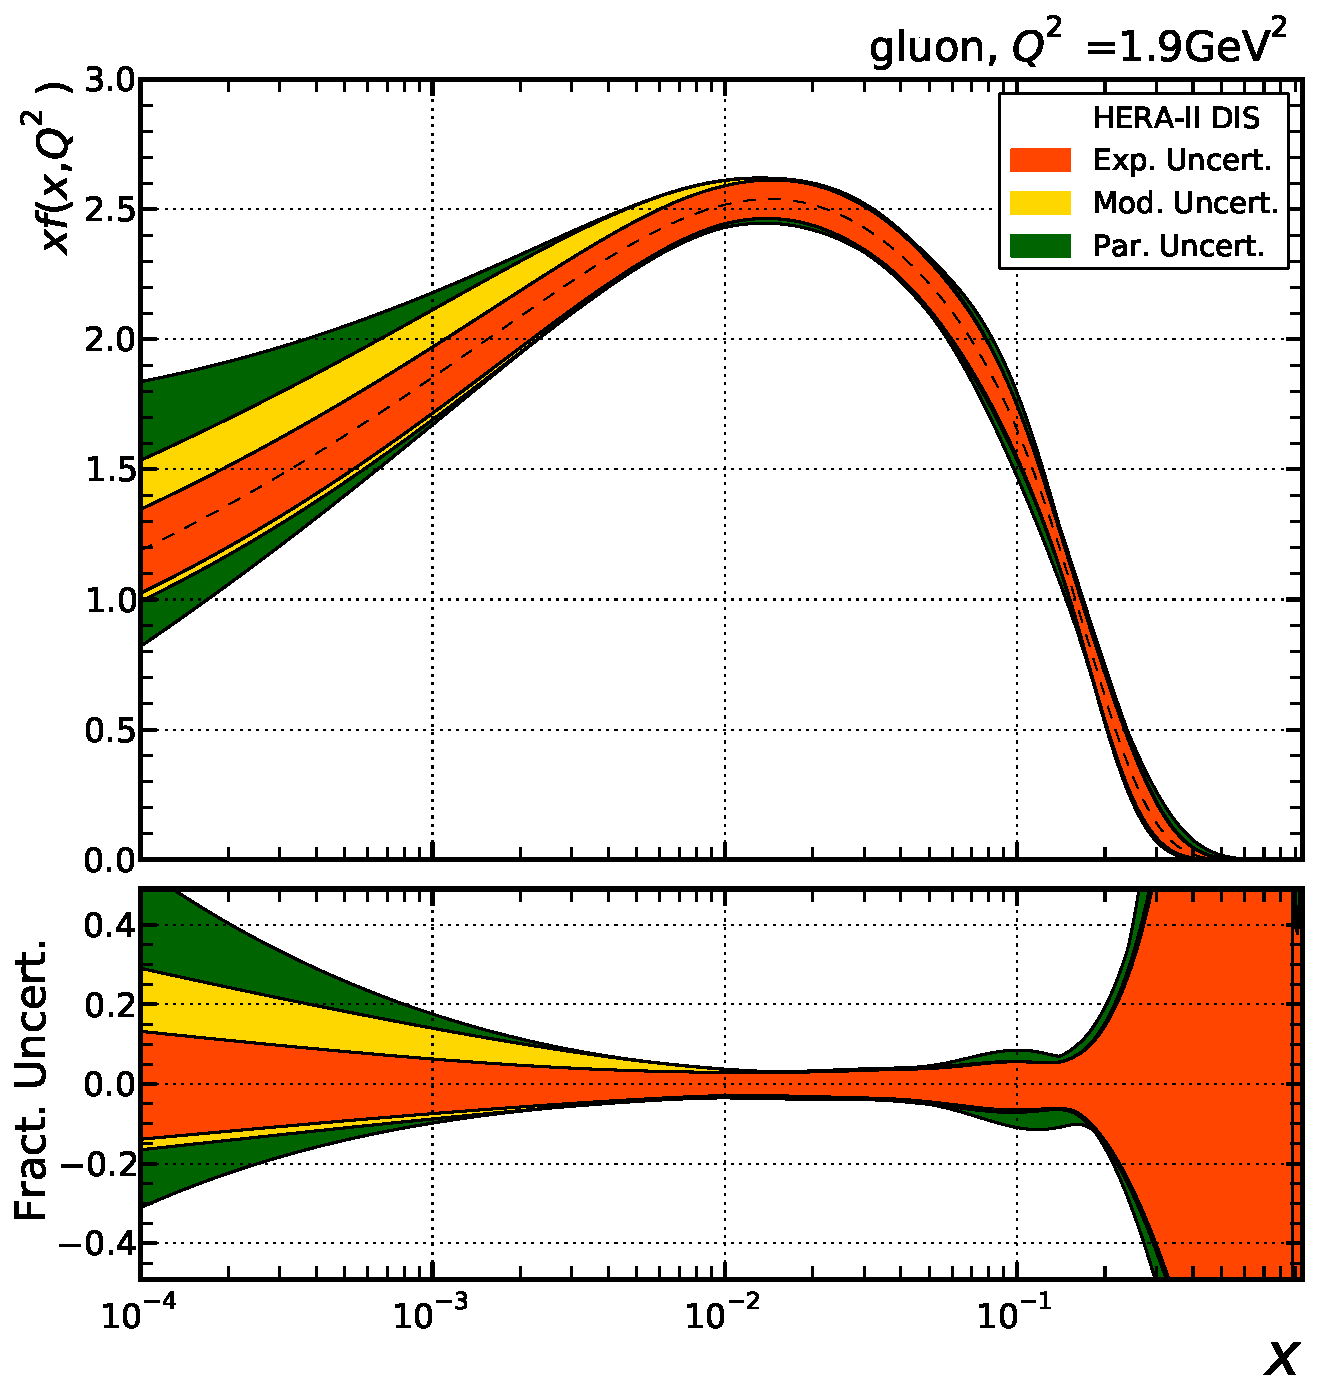
\includegraphics[width=0.48\textwidth]{figures/pdf_constraints/split_hera/HFTD_HERA_V017_EIG_0_1_9.pdf}\hfill%
  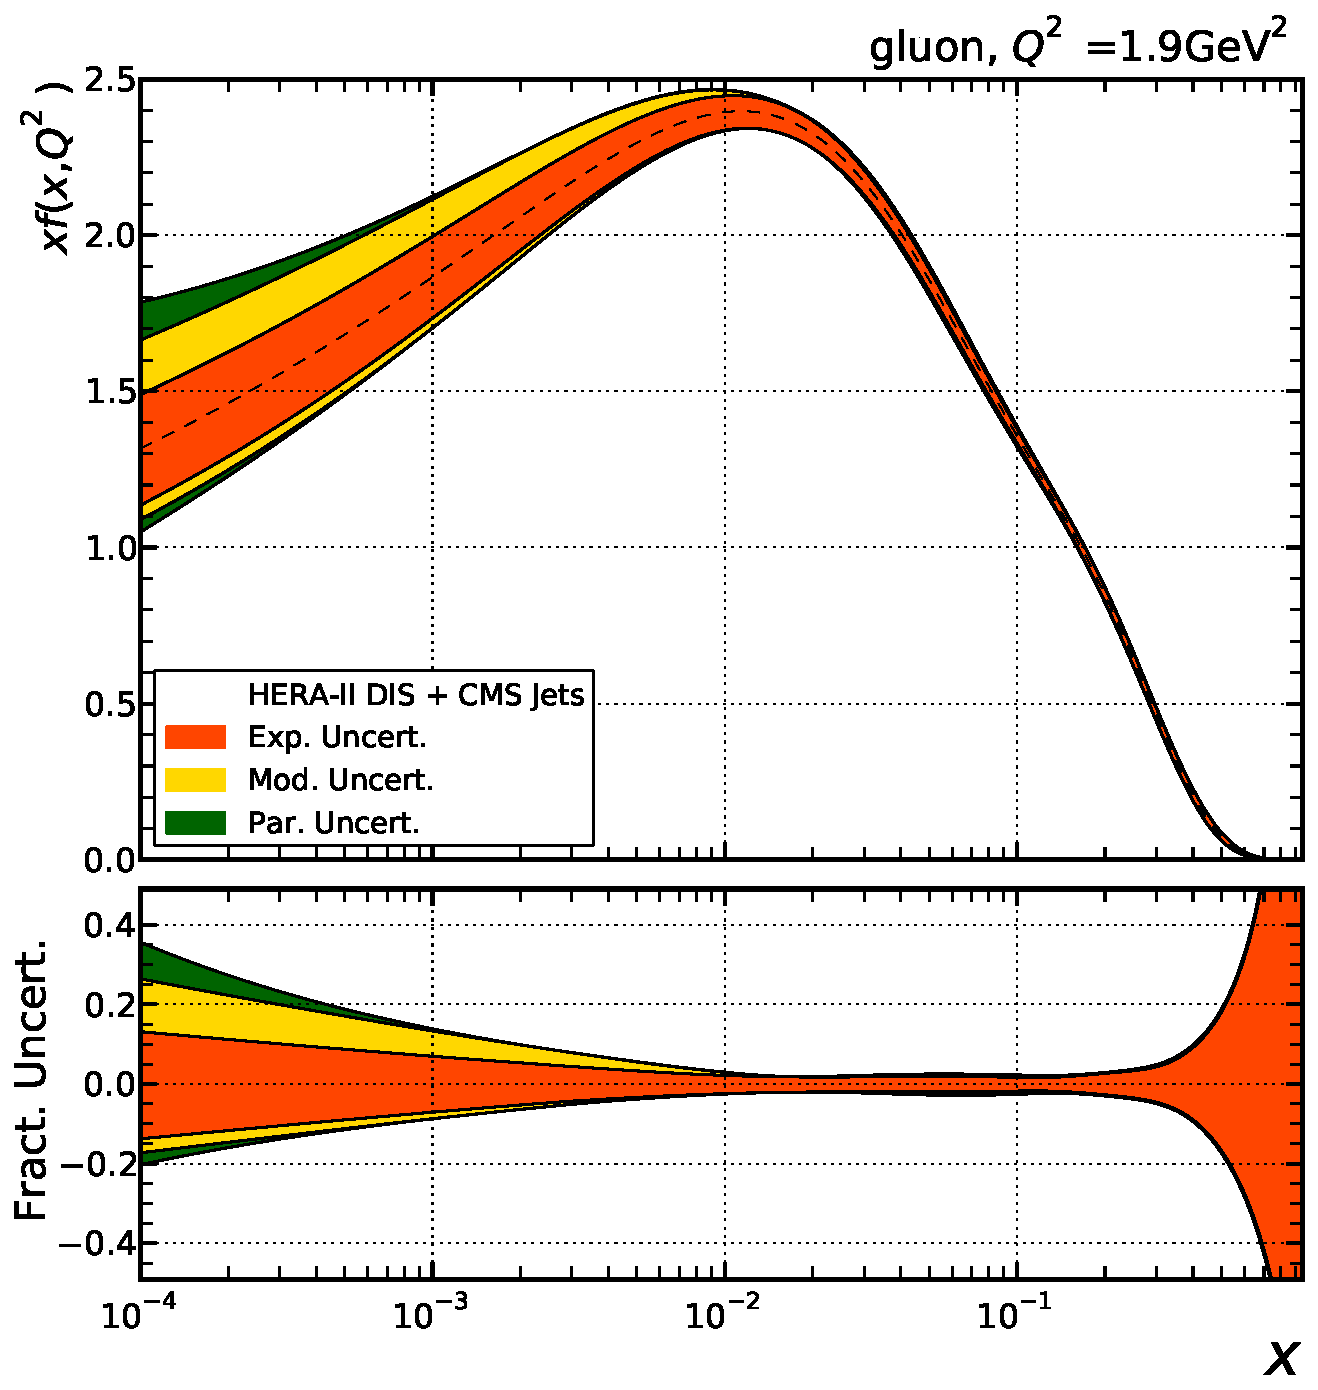
\includegraphics[width=0.48\textwidth]{figures/pdf_constraints/split_heracms/HFTD_HERACMSTDJETS_V017_EIG_0_1_9.pdf}
  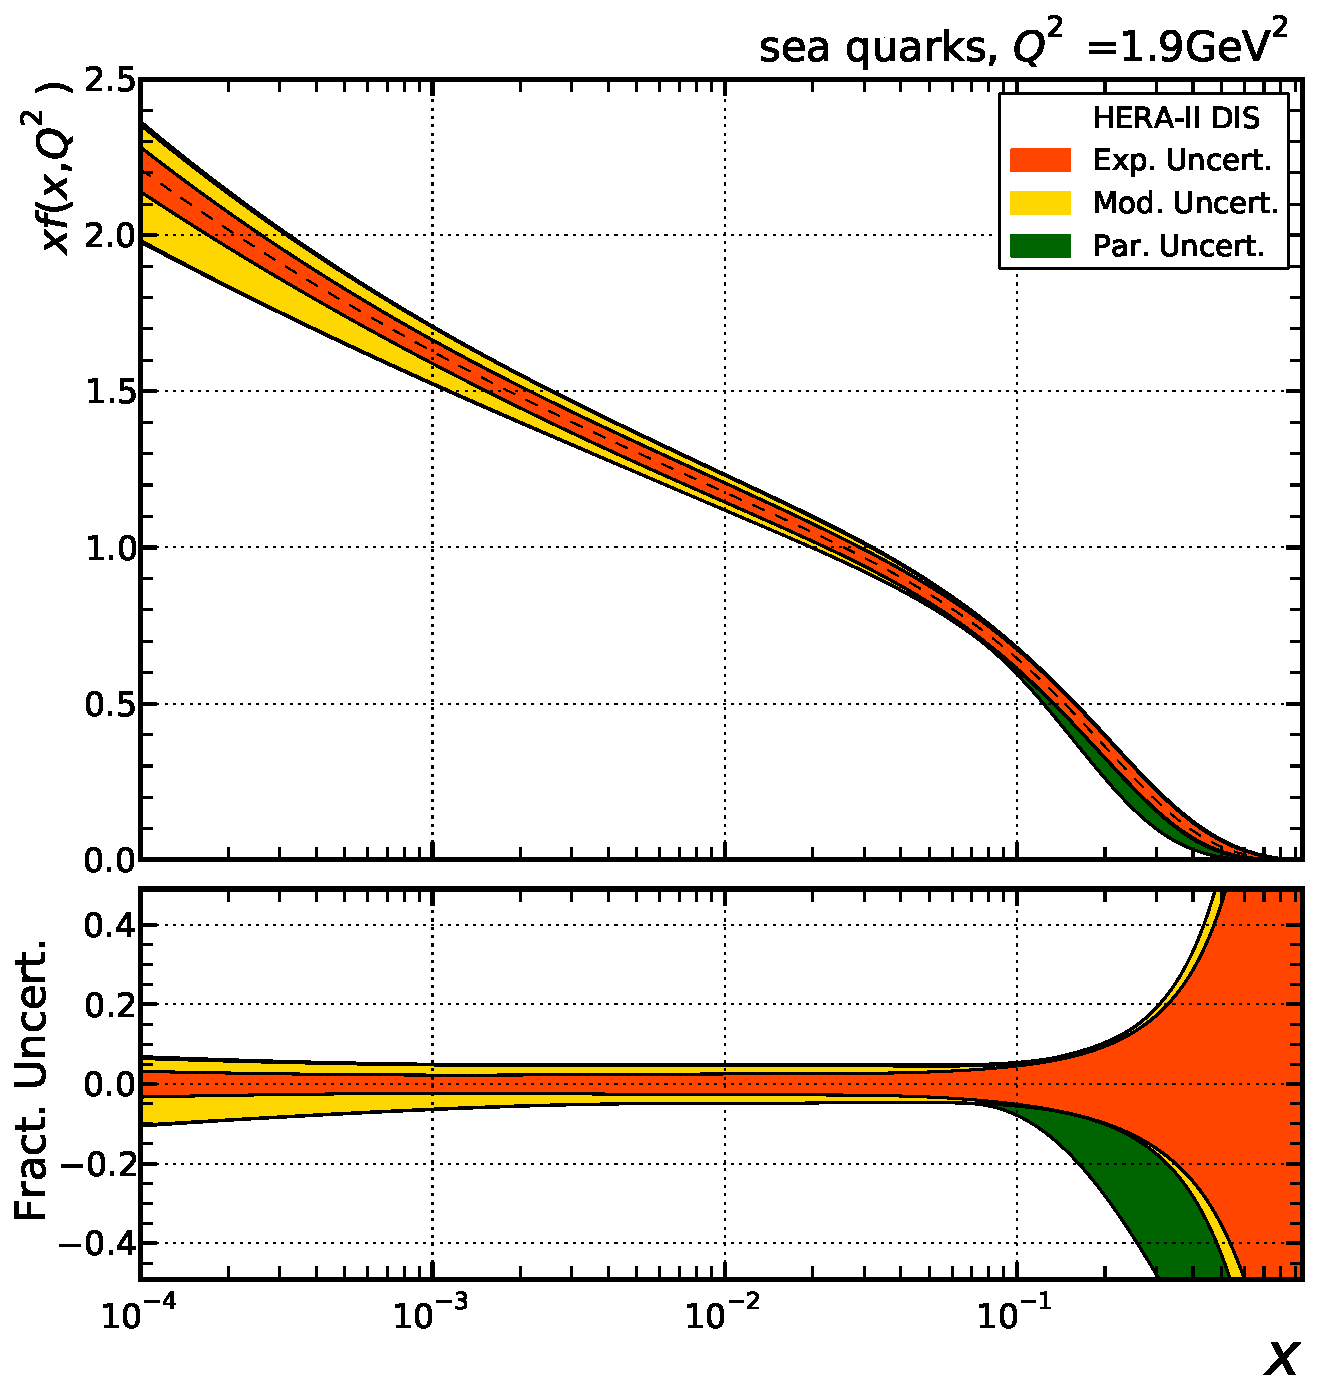
\includegraphics[width=0.48\textwidth]{figures/pdf_constraints/split_hera/HFTD_HERA_V017_EIG_9_1_9.pdf}\hfill%
  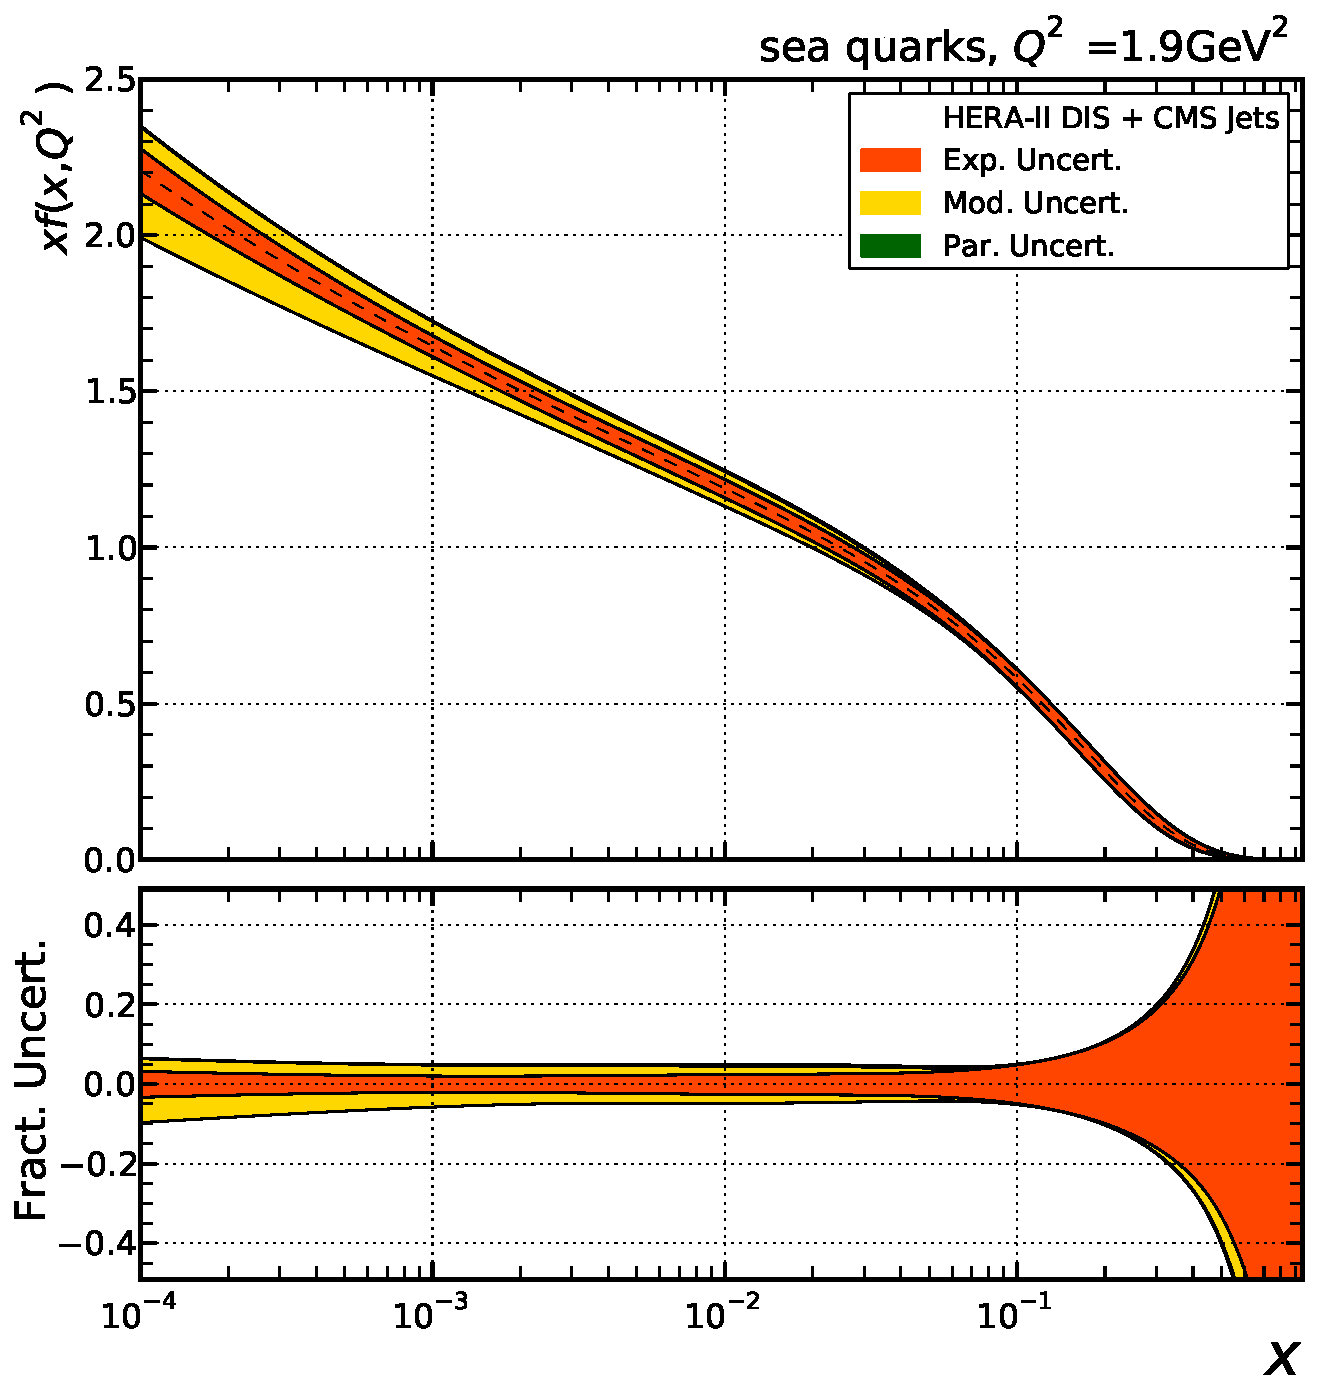
\includegraphics[width=0.48\textwidth]{figures/pdf_constraints/split_heracms/HFTD_HERACMSTDJETS_V017_EIG_9_1_9.pdf}
  \caption{}
  \label{fig:pdfconstraints:split:gluonqsea:19}
\end{figure}

\begin{figure}[tbp]
  \centering
  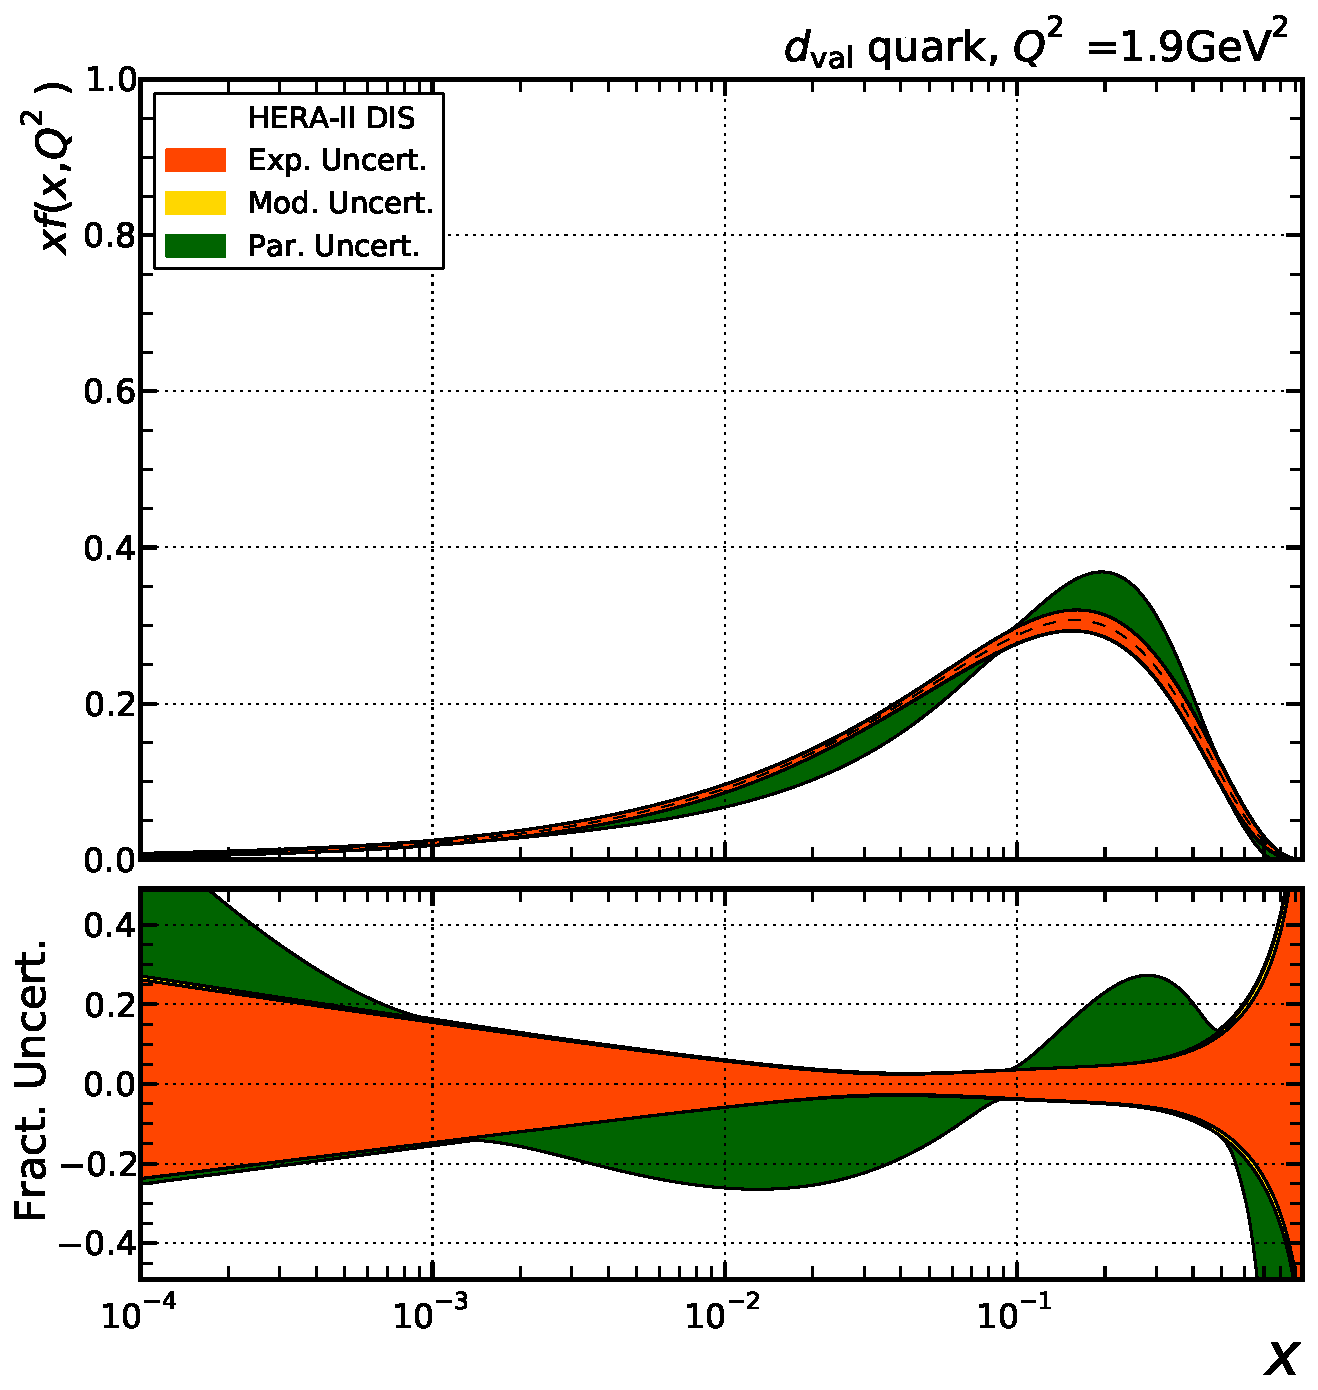
\includegraphics[width=0.48\textwidth]{figures/pdf_constraints/split_hera/HFTD_HERA_V017_EIG_7_1_9.pdf}\hfill%
  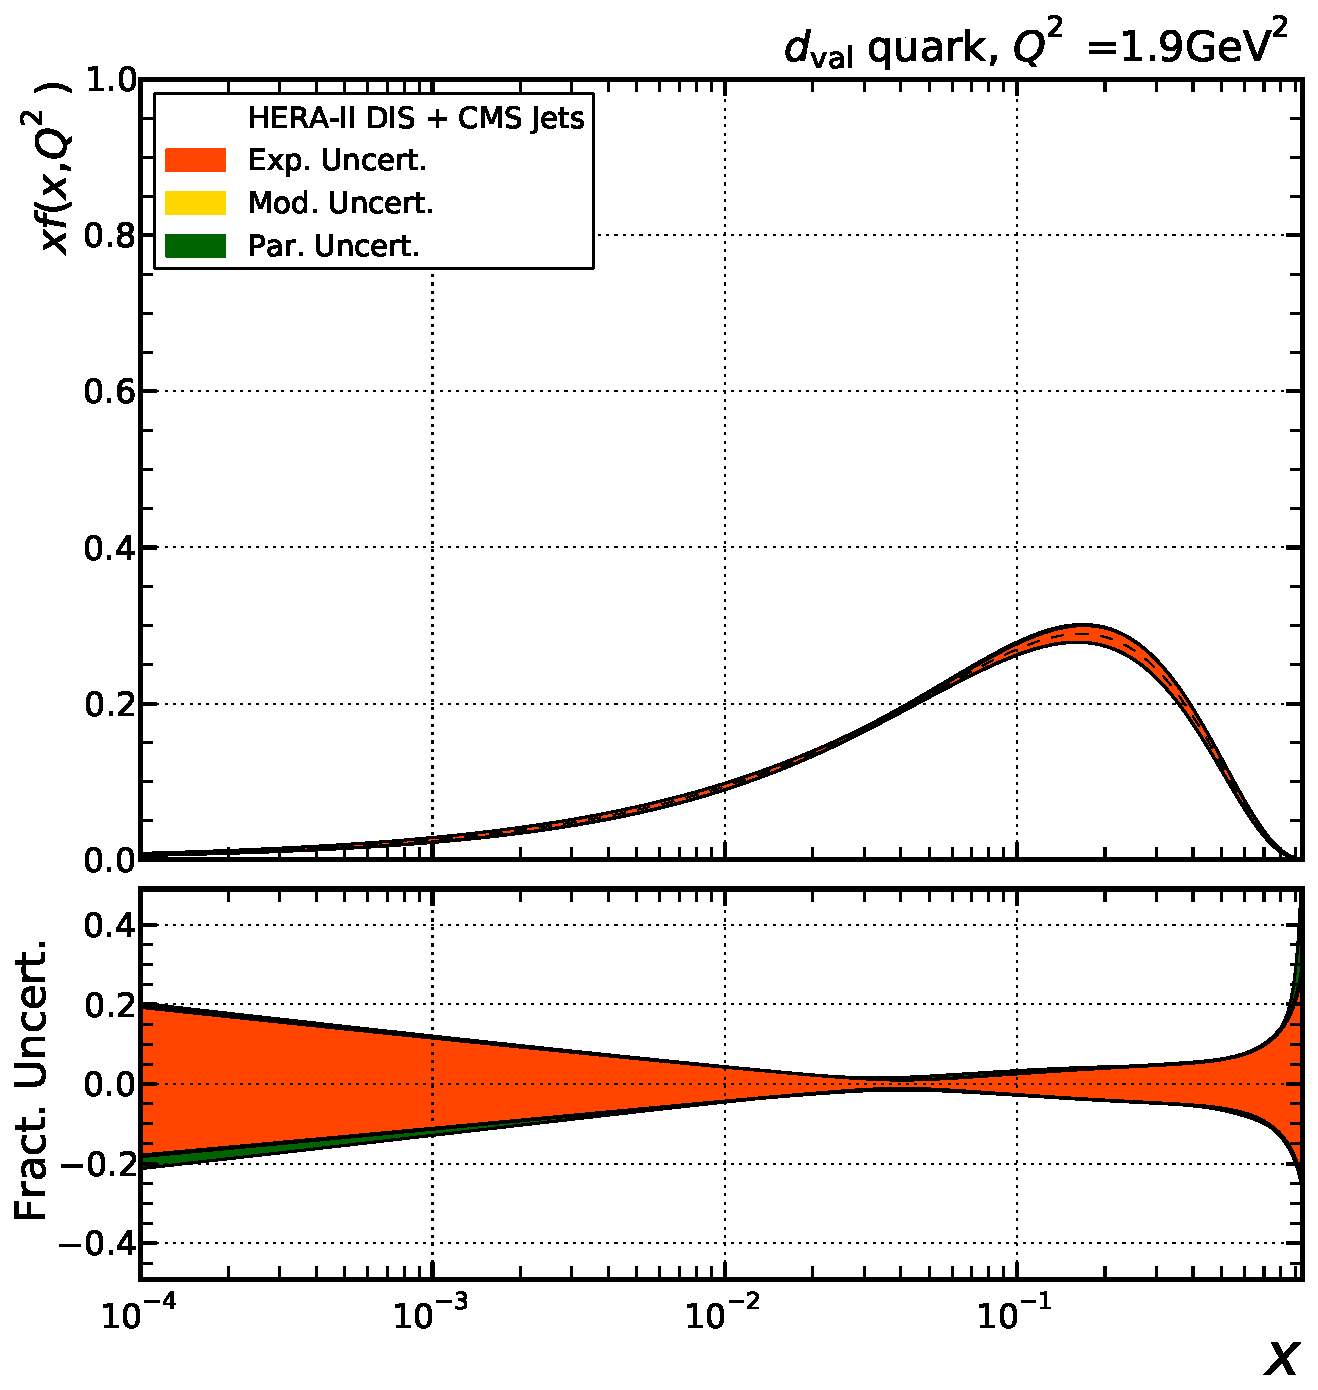
\includegraphics[width=0.48\textwidth]{figures/pdf_constraints/split_heracms/HFTD_HERACMSTDJETS_V017_EIG_7_1_9.pdf}
  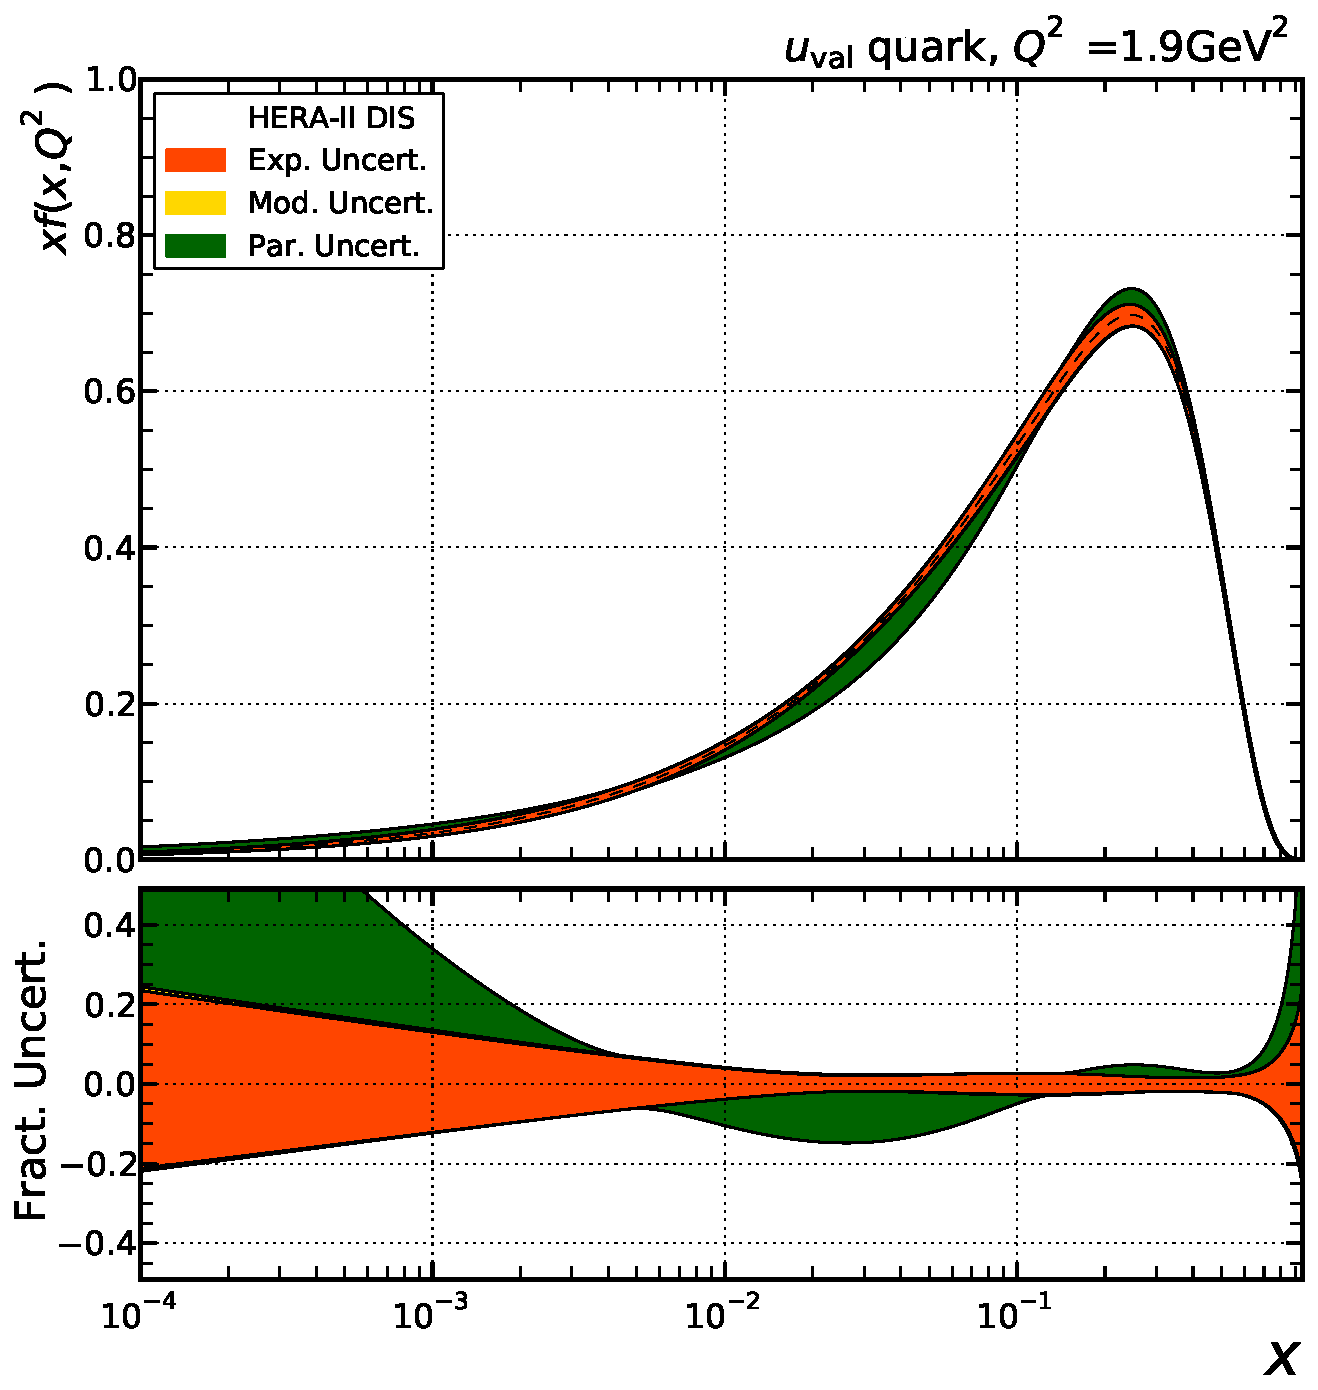
\includegraphics[width=0.48\textwidth]{figures/pdf_constraints/split_hera/HFTD_HERA_V017_EIG_8_1_9.pdf}\hfill%
  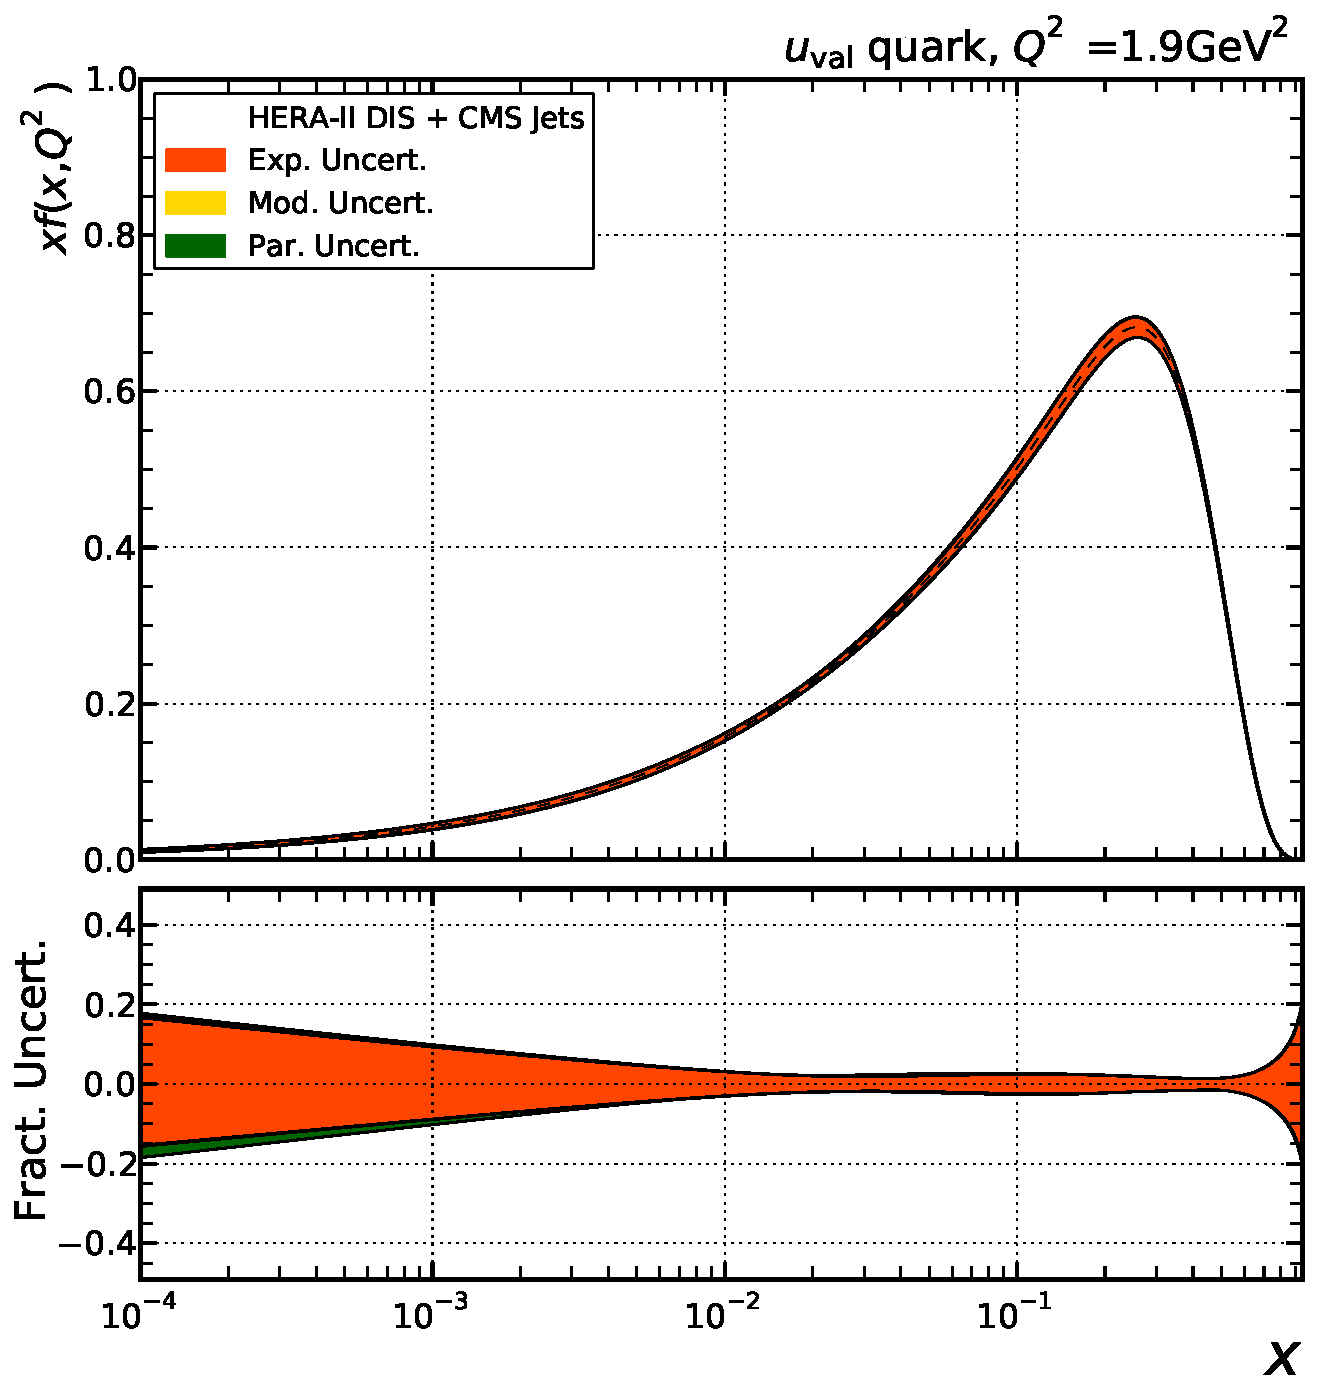
\includegraphics[width=0.48\textwidth]{figures/pdf_constraints/split_heracms/HFTD_HERACMSTDJETS_V017_EIG_8_1_9.pdf}
  \caption{}
  \label{fig:pdfconstraints:split:dvaluval:19}
\end{figure}


%
%
% For a direct comparison
% Figs.~\ref{fit:cmsjets2011:directcomparison:fitscale}
% and~\ref{fit:cmsjets2011:directcomparison:10000} display for all PDFs
% at both scales, $Q^2 = 1.9 \GeVsq$ and $10^4 \GeVsq$, the fit results
% and total uncertainties with and without CMS jet data on top of each
% other. Finally, Fig.~\ref{fit:cmsjets2011:overview} shows an overview
% of the gluon, sea, u valence, and d valence distributions at the
% starting scale of $Q^2 = 1.9 \GeVsq$ within one plot.
\begin{figure}[tbp]
  \centering
  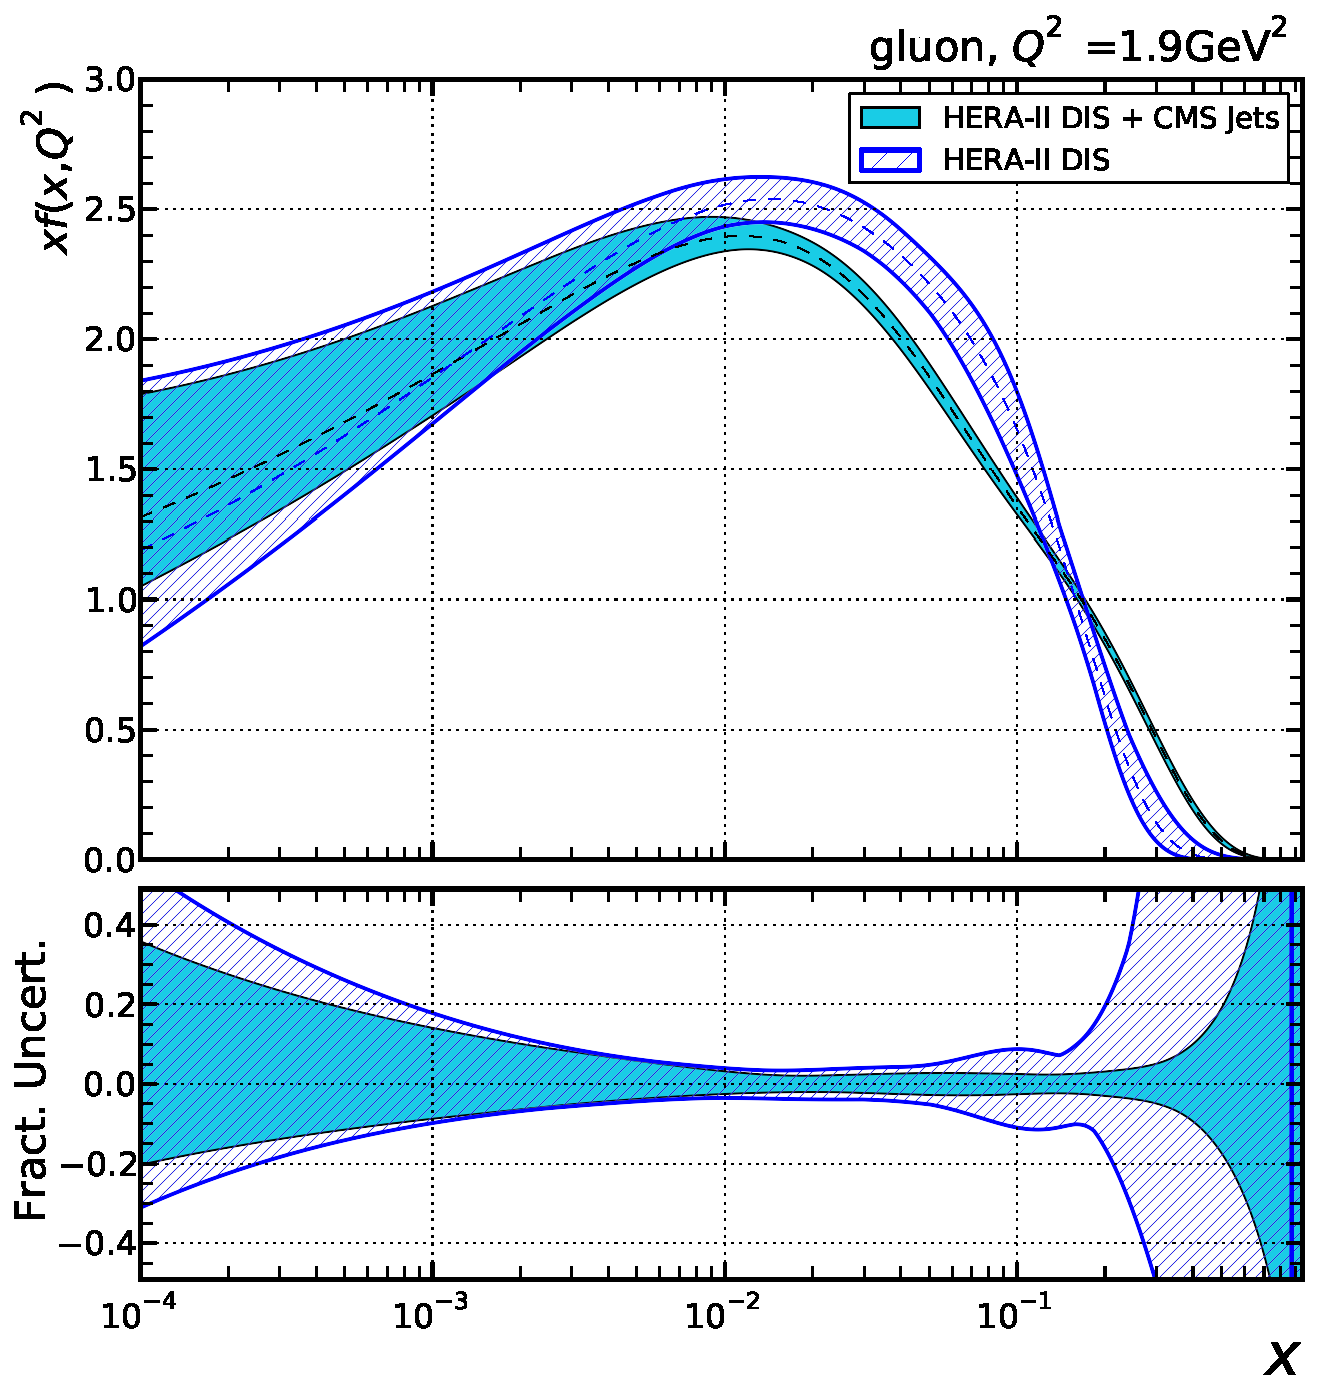
\includegraphics[width=0.48\textwidth]{figures/pdf_constraints/direct/HFTD_HERACMSTDJETS_V017_EIG_0_1_9.pdf}\hfill%
  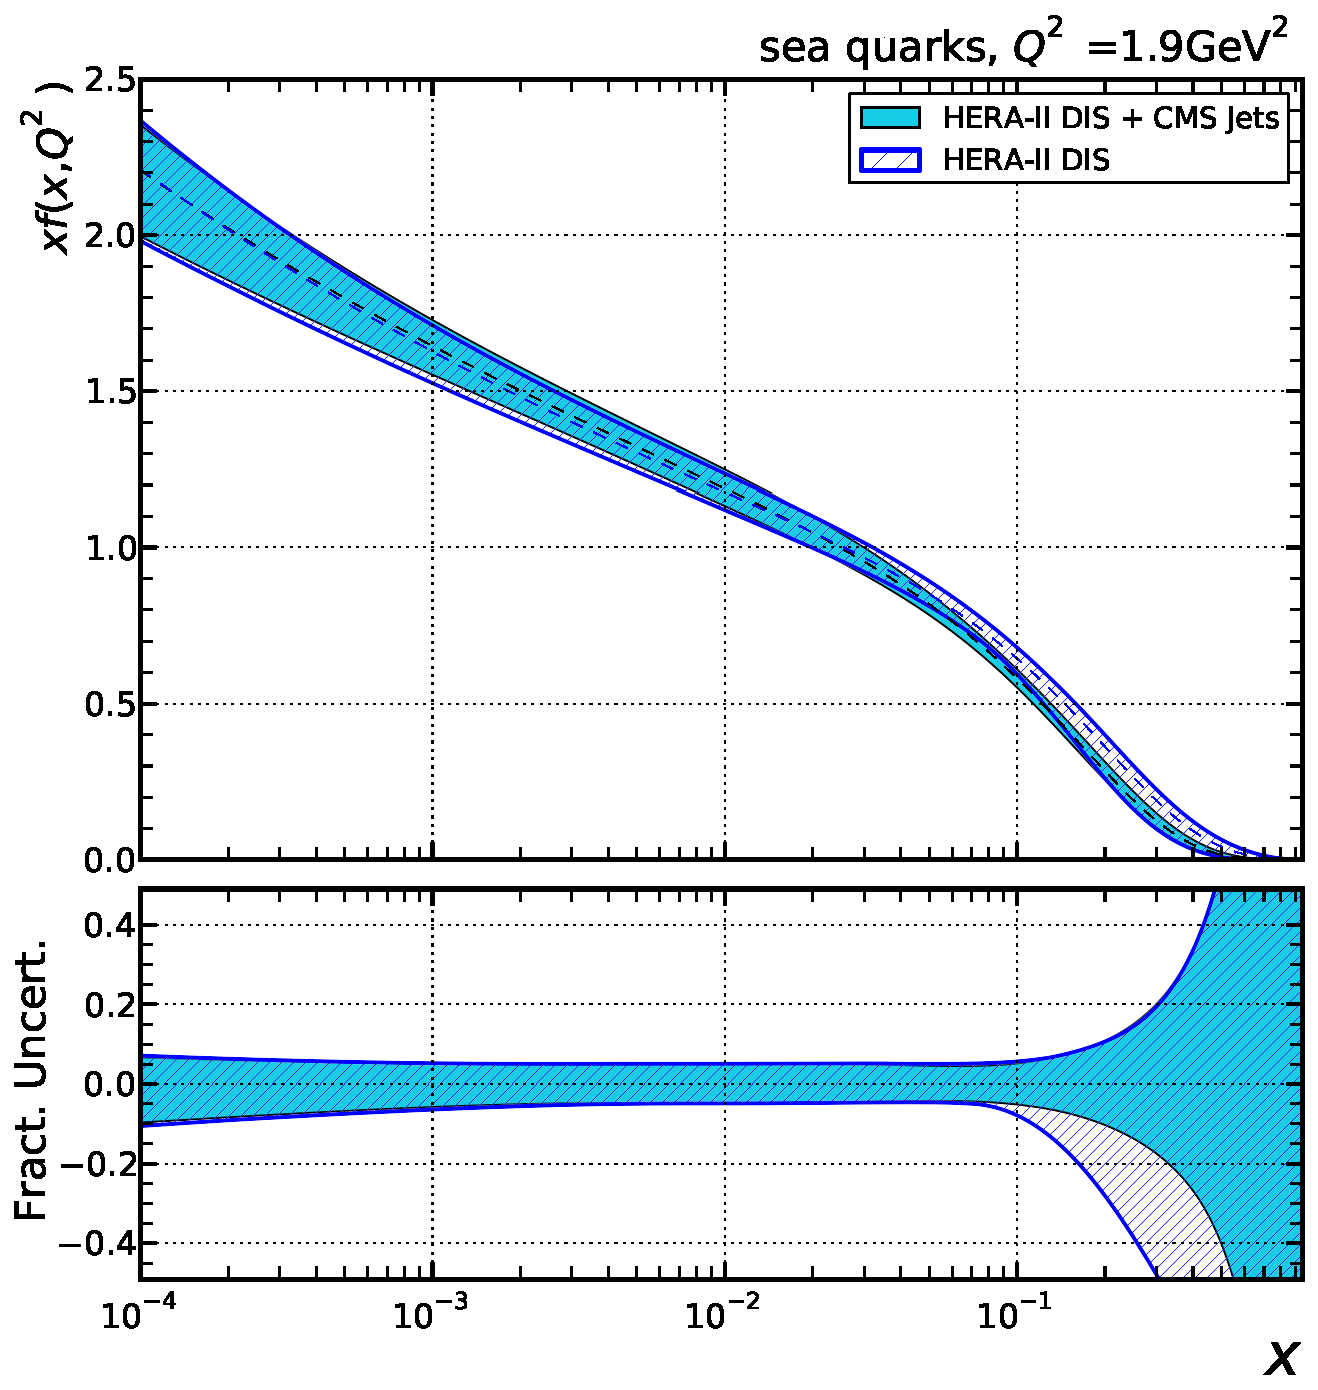
\includegraphics[width=0.48\textwidth]{figures/pdf_constraints/direct/HFTD_HERACMSTDJETS_V017_EIG_9_1_9.pdf}
  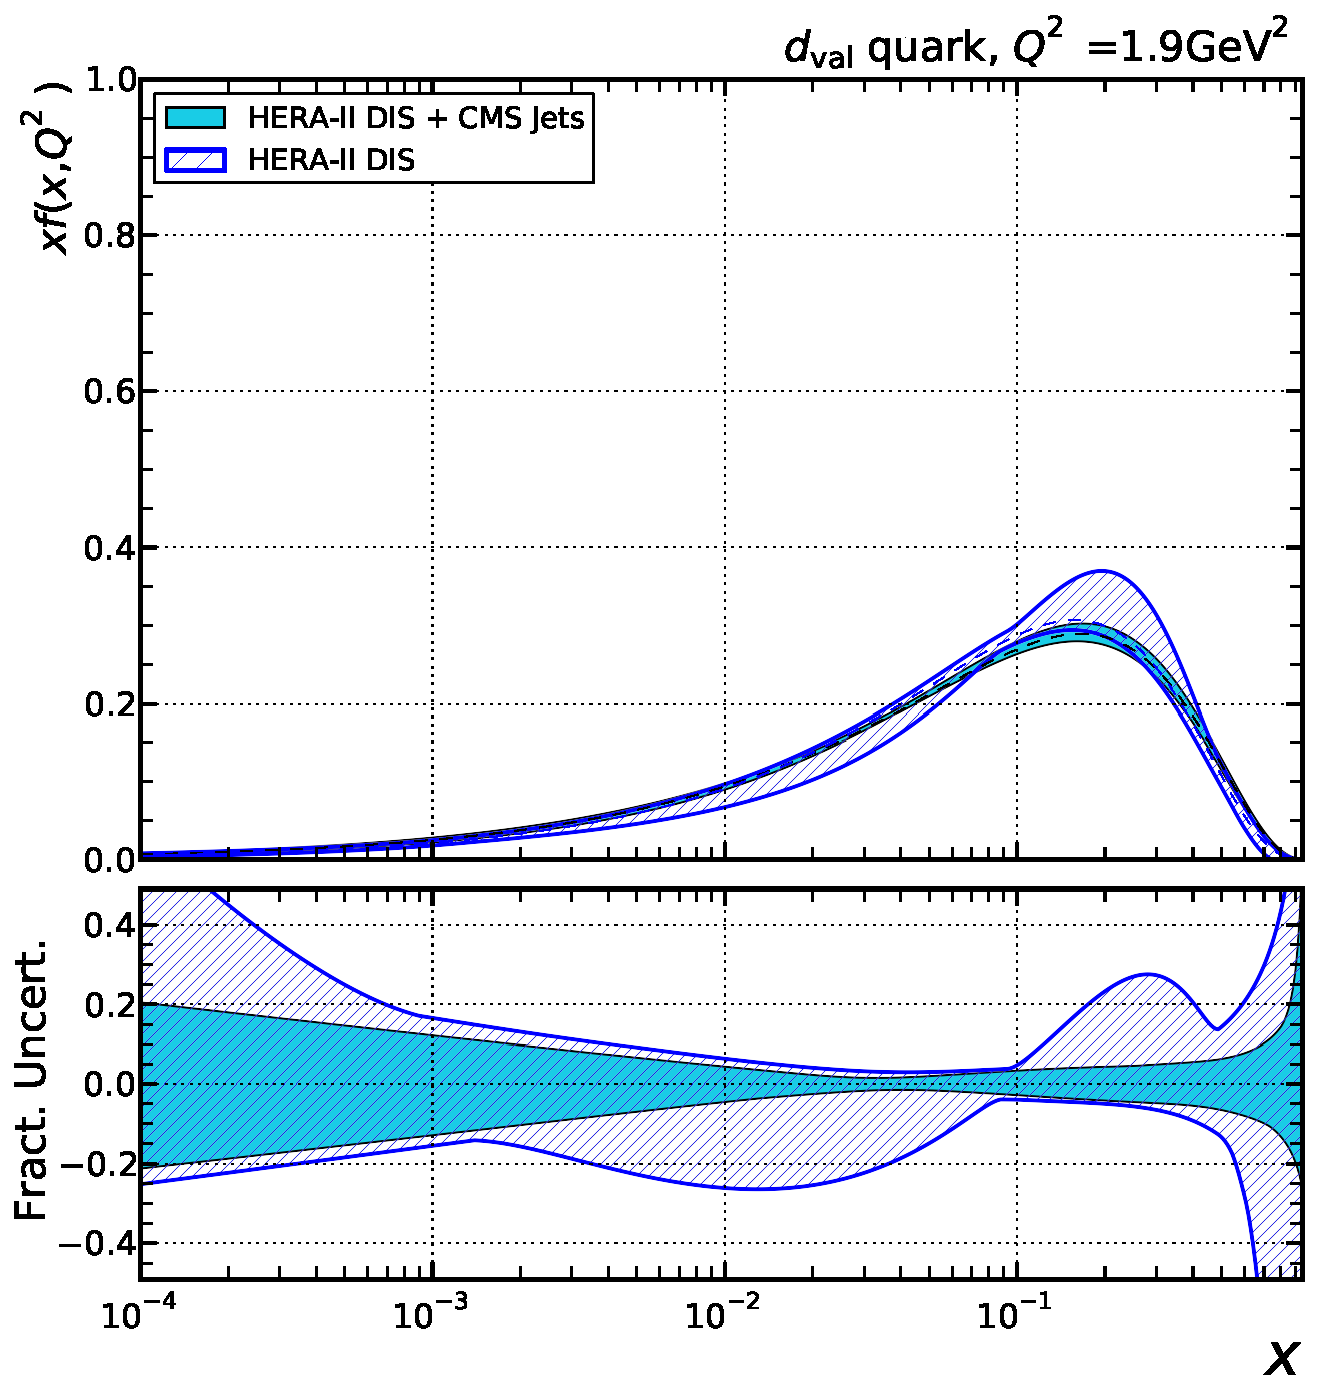
\includegraphics[width=0.48\textwidth]{figures/pdf_constraints/direct/HFTD_HERACMSTDJETS_V017_EIG_7_1_9.pdf}\hfill%
  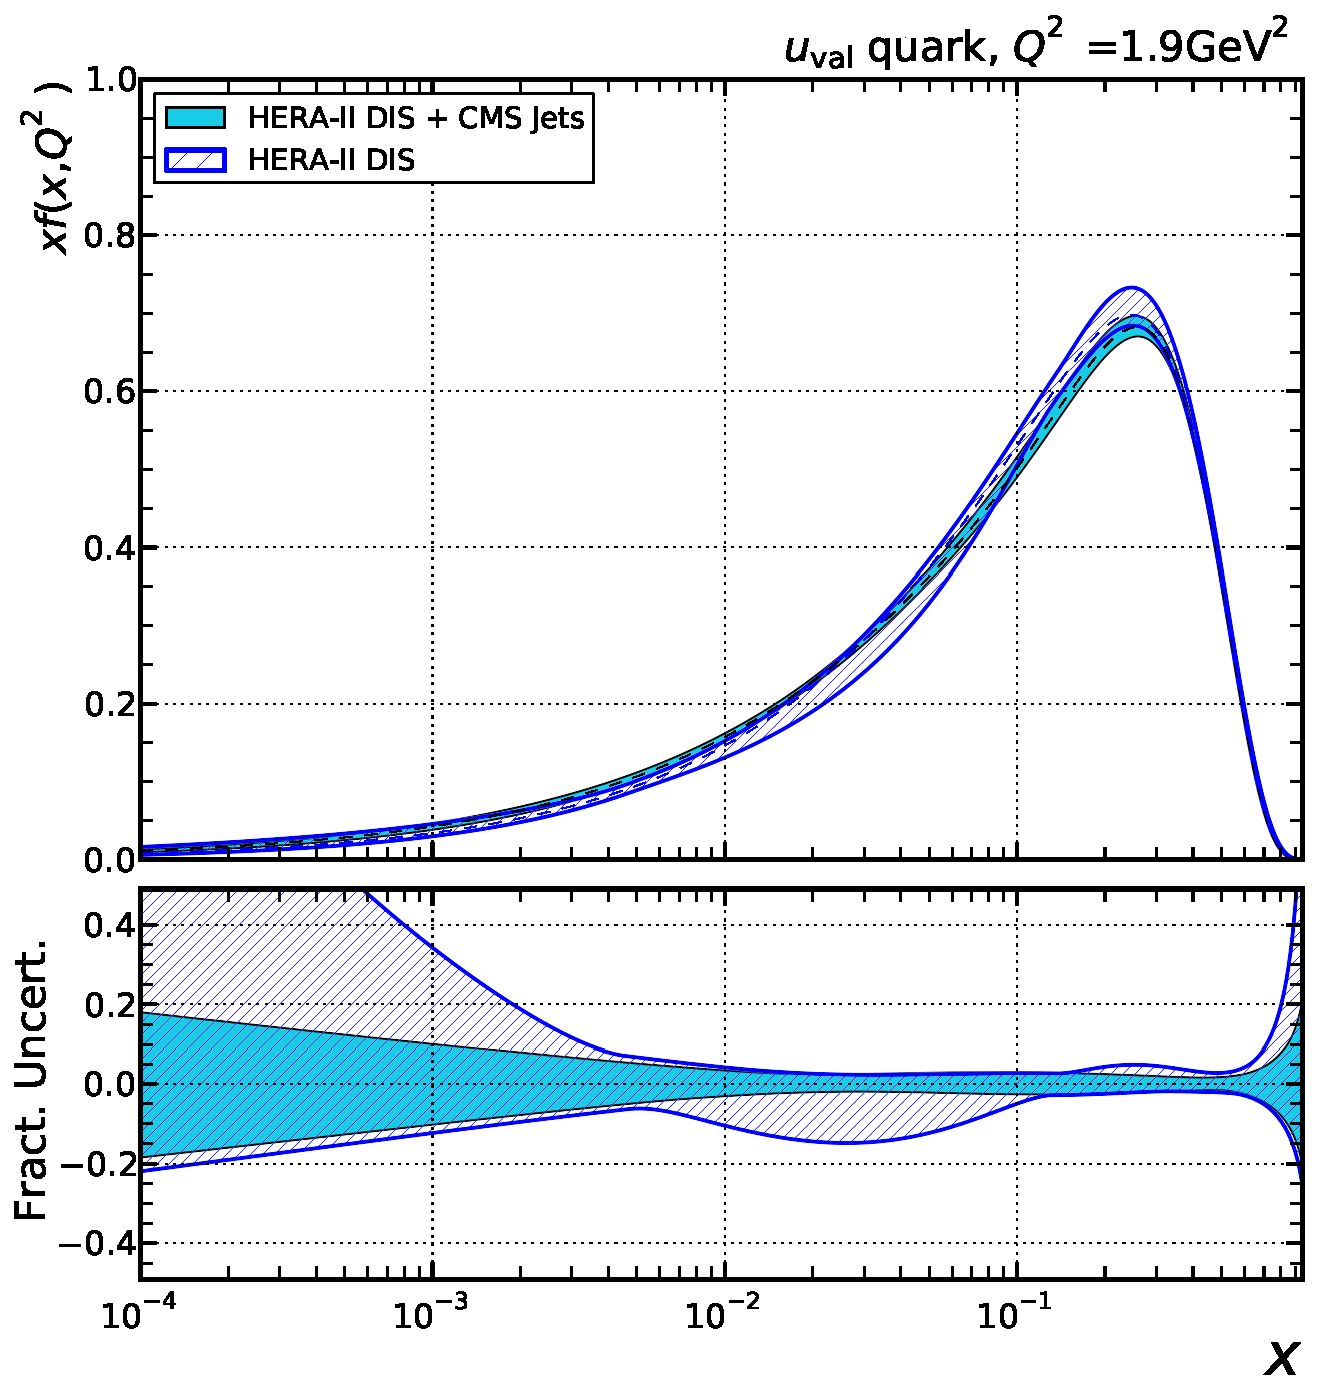
\includegraphics[width=0.48\textwidth]{figures/pdf_constraints/direct/HFTD_HERACMSTDJETS_V017_EIG_8_1_9.pdf}
  \caption{}
  \label{fig:pdfconstraints:direct:19}
\end{figure}


%
% At the same time CMS jet data favour a larger gluon PDF at high $x$
% compared to the DIS data alone. As expected, no improvement is
% exhibited in the low-$x$ region, where the gluon is well constrained
% by the HERA data through scaling violations.
%
% It can also be seen that the parameterization and model uncertainties
% of the up- and down-quark distributions are reduced for $x >
% 0.3$. This is expected from the correlations, studied in
% Fig.~\ref{fig:correlation_pdf_xs_gqq}, where the quark distributions
% are constrained via the $qq$ contribution to jet production at high
% \yabs and \pt.
%
% Considering the significant increase in the u valence uncertainty
% exhibited in the low-$x$ region of
% Fig.~\ref{fit:cmsjets2011:directcomparison:fitscale} one has to
% remember that a more flexible parameterization is used than for the
% original HERAPDF1.0 fits and that in this region the contribution of
% the u valence quarks is very small. Through the QCD sum rules better
% constraints at high $x$ can then counterintuitively lead to larger
% uncertainties at low $x$, if this region is not sufficiently
% constrained by other data. In fact, the experimental uncertainty is
% reduced and only the model and parameterization uncertainties have
% become larger for this region, which is clearly visible from
% Fig.~\ref{fit:cmsjets2011:seauvdv:fitscale}.
%
% Inclusive DIS data alone are not sufficient to disentangle effects on
% cross section predictions from changes in the gluon distribution or
% the strong coupling constant at the same time. Therefore the strong
% coupling constant was always fixed to be $\alpsmz= 0.1176$ in all the
% presented results as in the original HERAPDF1.0 derivation. Including
% the CMS jet data this constraint can be dropped giving similar PDFs
% with, of course, larger uncertainties than previously. Direct
% comparisons of fits with and without the CMS data are not possible in
% this case, because the fitting procedure does not converge anymore
% with inclusive DIS data alone when \alpsmz is considered as a free
% parameter. %

% Including the CMS jet data the strong coupling constant is determined
% to be $\alpsmz = 0.1192\,^{+0.0017}_{-0.0015}$, where the uncertainty
% accounts for the experimental uncertainties of the inclusive HERA DIS
% and CMS jet data, and the NP uncertainties.
